\documentclass[compress,12pt]{beamer}
\usepackage{caption}
\usepackage{subcaption}
\usetheme{Arguelles}
\usepackage{color}
\usepackage{tcolorbox}
\usepackage{xcolor}

\newcommand{\myRed}[1]{\textcolor{red}{#1}}

\title{MATH 512 - Project 2}
\subtitle{}
\event{}
\date{}
\author{Wasif Ahmed, Haoxiang Deng, Jacob Fein-Ashley, Kanav Malhotra}


\begin{document}

\frame[plain]{\titlepage}

\section{Question 1}

\begin{frame}{Question 1 (a)}
      We use the \emph{Kolmogorov-Smirnov} test to test for the uniformity of the random numbers generated by the LCG. The test statistic is given by
      \begin{equation*}
            D_n = \max_{1 \leq i \leq n} \left( \frac{i}{n} - U_{(i)} \right) \vee \max_{1 \leq i \leq n} \left( U_{(i)} - \frac{i-1}{n} \right)
      \end{equation*}
      where $U_{(i)}$ is the $i$-th order statistic of the $U_i$'s. 
      
      \begin{itemize}
            \item $H_{\circ}$: the random numbers are uniformly distributed. 
      \end{itemize}
      
    \begin{tcolorbox}
      We find that $D_n = 0.0069$ and a \myRed{p-value of $0.708$}. This means that we fail to reject $H_{\circ}$ at the 5\% significance level and conclude that the random numbers \myRed{are uniformly distributed.}
    \end{tcolorbox}
\end{frame}

\begin{frame}{Question 1 (a)}
      \begin{figure}
            \centering
            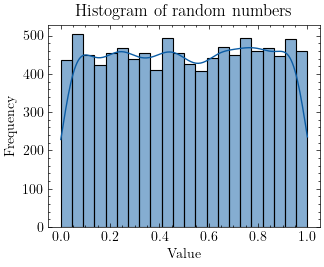
\includegraphics[scale=0.7]{imgs/1a.png}
      \end{figure}
\end{frame}

\begin{frame}{Question 1 (b)}

      Parameters: $a = 6, m = 11, x_0 = 3, c = 1$ and $n=10$
      \begin{itemize}
            \item The sequence is $\{3, 7, 9, 10, 5, 8, 4, 2, 1, 6\}$
            \item The period is 1
            % \item What do you observe?
      \end{itemize}

      Parameters: $a = 6, m = 10, x_0 = 3, c = 1$ and $n=10$
      \begin{itemize}
            \item The sequence is $\{3, 8, 8, 8, 8, 8, 8, 8, 8, 8\}$
            \item The period is 2
            % \item  What do you observe?
      \end{itemize}
    \begin{tcolorbox}
    We notice that even a \emph{small} change in the parameters results in a seemingly non-random sample.
      \end{tcolorbox}
\end{frame}

\begin{frame}{Question 1 (c)}
      \begin{figure}
            \centering
            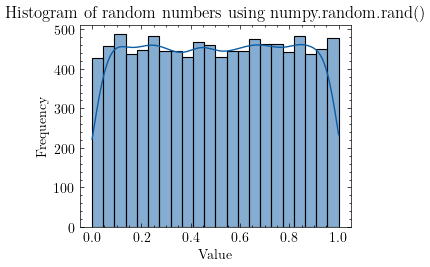
\includegraphics[scale=0.7]{imgs/1d.png}
      \end{figure}
\end{frame}

\begin{frame}{Question 1 (d)}
      \begin{figure}
            % put the histograms next to each other
            \centering
            \begin{subfigure}{0.45\textwidth}
                  \centering
                  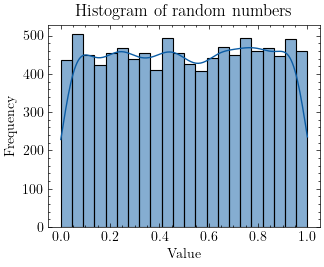
\includegraphics[scale=0.5]{imgs/1a.png}
            \end{subfigure}
            \begin{subfigure}{0.45\textwidth}
                  \centering
                  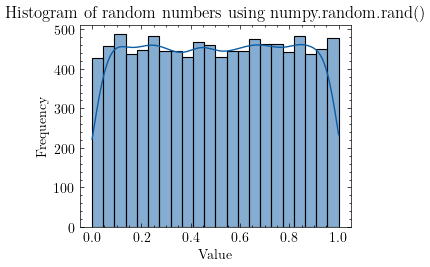
\includegraphics[scale=0.5]{imgs/1d.png}
            \end{subfigure}
      \end{figure}

      \begin{itemize}
            \item The two histograms look relatively similar, meaning both look relatively uniform.
      \end{itemize}
\end{frame}

\begin{frame}{Question 1 (e)}
      \begin{figure}
            \centering
            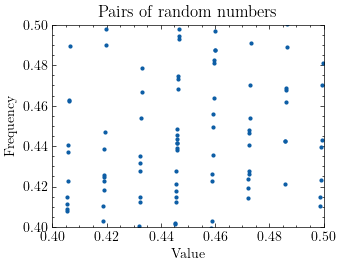
\includegraphics[scale=0.6]{imgs/pairs.png}
      \end{figure}
      \begin{itemize}
            \item The pairs of numbers seem to have a random pattern.
      \end{itemize}
\end{frame}

\begin{frame}{Question 1 (f)}
      Disadvantages of LCG:
      \begin{itemize}
      \begin{tcolorbox}
            \item It can appear random with the right set of parameters, but as we saw, it can get ``stuck'' in a loop.
            \item The randomness depends on the choice of parameters.
        \end{tcolorbox}
      \end{itemize}

    
\end{frame}

\section{Question 2}
\begin{frame}{Question 2}

%       # 𝑃(𝑋 = 𝑘) = {
% # 0.3 for 𝑘 = 1
% # 0.2 for 𝑘 = 2
% # 0.35 for 𝑘 = 3
% # 0.15 for 𝑘 = 4
\begin{align*}
      P(X = k) = \begin{cases}
            0.3 & \text{for } k = 1 \\
            0.2 & \text{for } k = 2 \\
            0.35 & \text{for } k = 3 \\
            0.15 & \text{for } k = 4
      \end{cases}
\end{align*}

      \begin{figure}
            \centering
            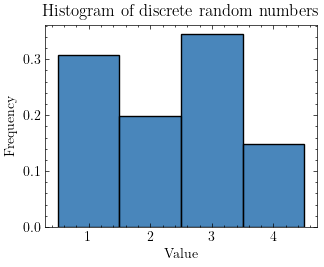
\includegraphics[scale=0.6]{imgs/discrete.png}
      \end{figure}
      
\end{frame}

\section{Question 3}
\begin{frame}{Question 3(a)}
     \begin{itemize}
         \item Time for generation: $0.0349$ seconds using NumPy's built-in function.
         \item Probability that $X < 50$: $0.00000000$.
     \end{itemize}
        \begin{align*}
                P(X < 50) &= \sum_{k=0}^{49} {100 \choose k} (0.8)^k (0.2)^{100-k} = {\color{red}0.00000000}
        \end{align*}
      
\end{frame}

\begin{frame}{Question 3(b)}
\centering
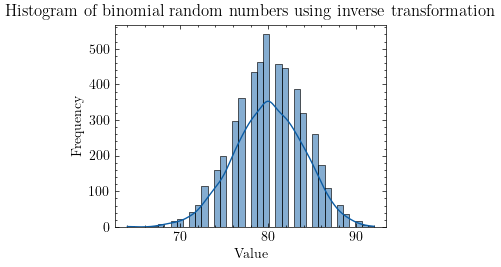
\includegraphics[scale=0.7]{imgs/binomialinverse.png}  \\
\begin{itemize}
    \item Time for generation: $0.0350$ seconds using the the inverse transform method.   
\end{itemize}
\end{frame}

\begin{frame}{Question 3(c)}
     The histograms and the times for generation for the inverse method and NumPy's random number generator are very similar. We are comparing {\color{red}$0.0349$} seconds to {\color{red}$0.0350$} seconds, which is a very small difference.
\end{frame}

\section{Question 4}
\begin{frame}{Question 4}
\centering
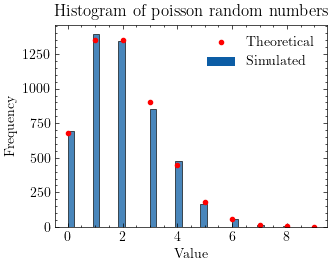
\includegraphics[scale=0.7]{imgs/poissonrv.png} 
\end{frame}

\section{Question 5}
\begin{frame}{Question 5}
\centering
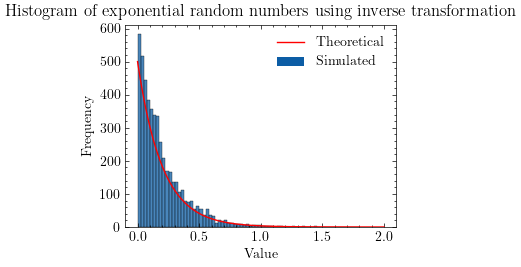
\includegraphics[scale=0.7]{imgs/exprv.png}
\end{frame}

\section{Question 6}
\begin{frame}{Question 6}
\centering
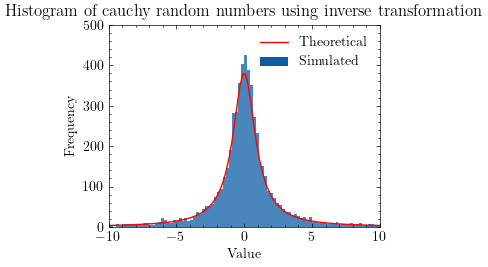
\includegraphics[scale=0.7]{imgs/cauchyrv.png}
\end{frame}

\section{Question 7}
\begin{frame}

With a repetition of $10000$ simulations, we find that {\color{red}the expectation is $1.00$} and {\color{red}the variance is $1.01$}.


We can calculate $\mathbb{E}[X]$ and $\mathbb{V}[X]$ exactly and compare them with our estimates. We have
\begin{align*}
    % expected value is 1
    \mathbb{E}[X] &= \sum_{i=1}^{100} i \cdot \frac{1}{100} = 1 \\
    % variance is 1
    \mathbb{V}[X] &= \sum_{i=1}^{100} (i - 1)^2 \cdot \frac{1}{100} - 1 = 1
\end{align*}

{\color{red}The estimates are very close to the exact values.} This is expected because the number of simulations is large.
\end{frame}

\section{Question 8}

\begin{frame}
    \begin{enumerate}
        \item Model the number of rolls needed as a geometric r.v.
        \[
         X \sim \text{Geometric}(p)
         \]
         where $p$ is the probability that all the possible outcomes have occurred at least once. 
        \item Calculate the probability \[
        p = \frac{6 \cdot 5 \cdot 4 \cdot 3 \cdot 2 \cdot 1}{6^6} = \frac{720}{46656} \approx 0.0154
         \]
        \item Calculate the expected value of $X$ as
        \[
        \mathbb{E}[X] = \frac{1}{p} = \frac{46656}{720} \approx 64.8
        \]
         The simulation gives us an estimate of $\mathbb{E}[X] \approx 64.8$. 
        \item Then, the variance of $X$ is\[
        \mathbb{V}[X] = \frac{1 - p}{p^2} = \frac{1 - 0.0154}{0.0154^2} \approx 4151.63
         \]
    \end{enumerate}

\end{frame}

\section{Question 9}
\begin{frame}{Question 9}
\centering
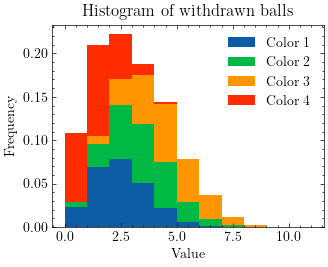
\includegraphics[scale=0.3]{imgs/balls.png}  
\end{frame}

\section{Question 10}
\begin{frame}{Question 10}
\centering
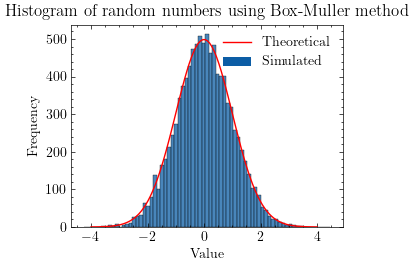
\includegraphics[scale=0.7]{imgs/boxmuller.png}  
\end{frame}
\begin{frame}
 \centering
 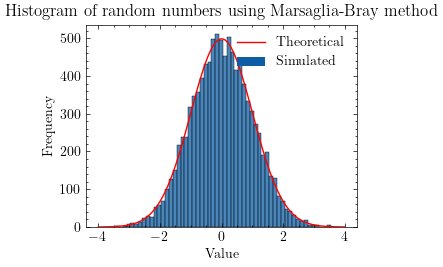
\includegraphics[scale=0.7]{imgs/marsagliabray.png}  \\
\end{frame}
\begin{frame}
 \centering
 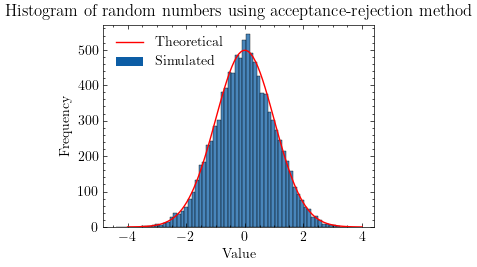
\includegraphics[scale=0.7]{imgs/acceptancerejection.png}  \\
\end{frame}
\begin{frame}
\centering
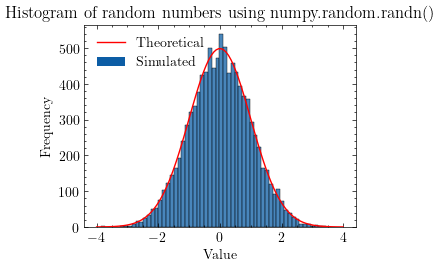
\includegraphics[scale=0.7]{imgs/numpyrandomrv.png}  \\
\begin{tcolorbox}
    All of the methods are very close to the theoretical normal distribution.  
\end{tcolorbox}

\end{frame}



\End
\begin{frame}[plain,standout]
      \centering
      Questions?
\end{frame}

\end{document}
